\chapter{Reference}

\section*{Possible appendices topics}

Hello, World.

\begin{figure}[h]
	\centering
	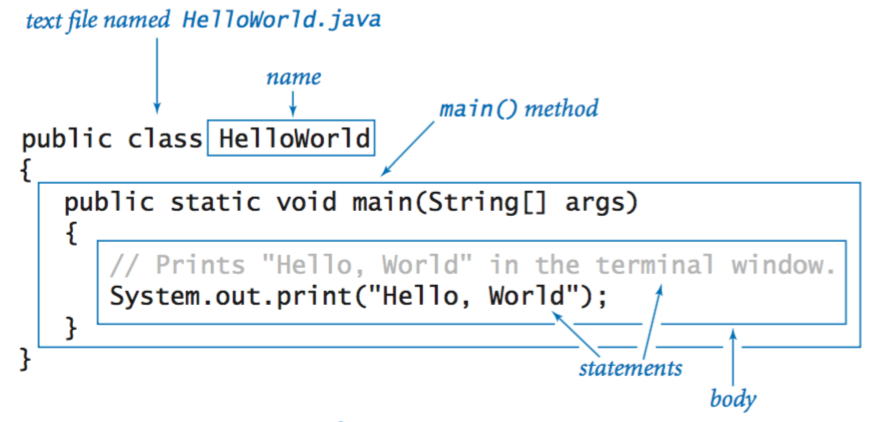
\includegraphics[width=0.85\textwidth]{images/hello_world_description}
	\label{fig:hello_world_description}
\end{figure}

Edit, compile, execute

\begin{figure}[h]
	\centering
	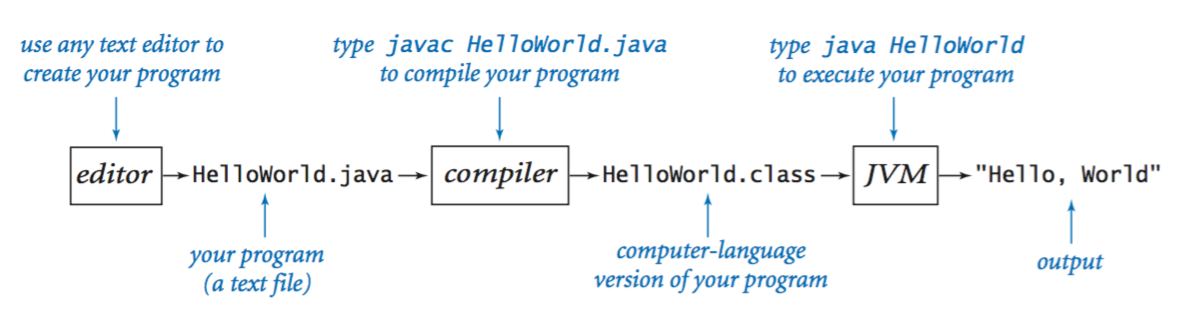
\includegraphics[width=0.85\textwidth]{images/edit_compile_execute}
	\label{fig:edit_compile_execute}
\end{figure}

Built-in data types

\begin{figure}[h]
	\centering
	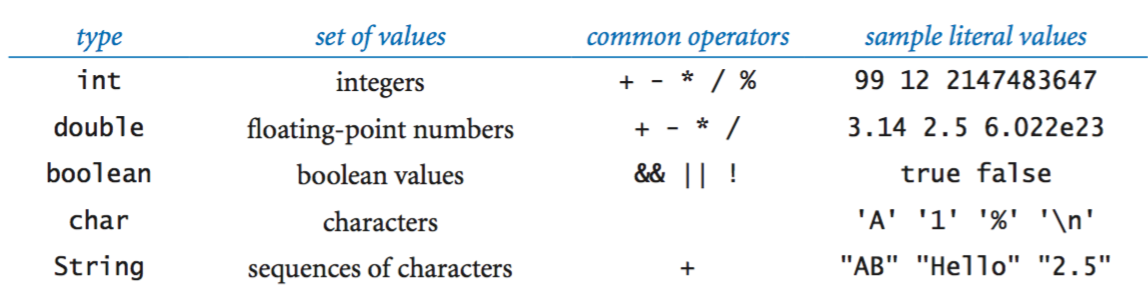
\includegraphics[width=0.85\textwidth]{images/data_types}
	\label{fig:data_types}
\end{figure}

Booleans

\begin{figure}[h]
	\centering
	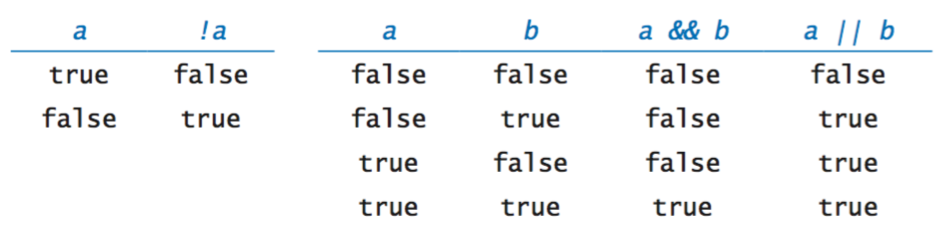
\includegraphics[width=0.85\textwidth]{images/booleans}
	\label{fig:booleans}
\end{figure}

Printing

System.out.print() is for regular printing
System.out.println() is same as System.out.print() but adds a newline
System.out.printf() prints \textbf{f}ormatted text, so you can easily insert data types inside a string and specify things like how many decimals should go after numbers. 
\begin{tabular}{|l|l|}
\hline
Format Specifier & Effect\\
\hline
\%s,\%S & Formats String\\
\%f & Formats floating point (precision provided between \% and f)\\
\%d & Formats integer\\
\%c & Formats character\\
\%b, \%B & Formats Boolean\\
\hline
\end{tabular}

Example: 

\begin{code}
System.out.printf("%.3f\n%.4f%d\n", 1.252525, 1.353535, 3);
\end{code}

prints 

\begin{code}
1.253
1.35353
\end{code}

\ja{todo: Scanners}

\ja{Cite https://introcs.cs.princeton.edu/java/11cheatsheet/}

\begin{itemize}

	\item Comparing floating point numbers.
	\item Type conversion.
	\item Useful math functions, e.g. \ic{min()}, \ic{log}.

\end{itemize}

\section{Java Reserved Words}

TODO: fill this in

\section{Common Java packages}\label{appendix:packages}

Descriptions from: \url{https://docs.oracle.com/javase/8/docs/api/java/util/package-summary.html}.

TODO: What about interfaces such as List or other implementations such as LinkedList (vs. ArrayList)? What about more advanced data structures like maps? More granular types like \ic{java.lang.Long}?

\begin{fullwidth}
\begin{center}
\begin{tabularx}{\linewidth}{ l X }
\ic{java.lang.*} & Provides classes that are fundamental to the design of the Java programming language.
\\\\
\ic{java.lang.Object} & Class \ic{Object} is the root of the class hierarchy. Every class has \ic{Object} as a superclass. All objects, including arrays, implement the methods of this class.
\\\\
\ic{java.lang.Double} & The \ic{Double} class wraps a value of the primitive type \ic{double} in an object.
\\\\
\ic{java.lang.Integer} & The \ic{Integer} class wraps a value of the primitive type \ic{int} in an object.
\\\\
\ic{java.lang.Long} & The \ic{Long} class wraps a value of the primitive type \ic{long} in an object.
\\\\
\ic{java.lang.Math} & The class \ic{Math} contains methods for performing basic numeric operations such as the elementary exponential, logarithm, square root, and trigonometric functions.
\\\\
\ic{java.lang.Random} & An instance of this class is used to generate a stream of pseudorandom numbers.
\\\\
\ic{java.lang.String} & The String class represents character strings.
\\\\
\ic{java.lang.System} & The \ic{System} class contains several useful class fields and methods, most notably the \ic{out} field's \ic{println} method. It cannot be instantiated.
\\
\hline
\ic{java.util.*} & Contains the collections framework, legacy collection classes, event model, date and time facilities, internationalization, and miscellaneous utility classes (a string tokenizer, a random-number generator, and a bit array).
\\\\
\ic{java.lang.ArrayList} & An ordered collection (also known as a \emph{sequence}).
\\\\
\ic{java.util.Scanner} & A simple text scanner which can parse primitive types and strings using regular expressions.
\\
\hline
\ic{java.io} & \text{}
\end{tabularx}
\end{center}
\end{fullwidth}